\documentclass[aspectratio=169, 10pt]{beamer}
\usepackage{amsmath}
\usepackage{amsfonts}
\usepackage{hyperref}
\usepackage{tikz}
\usetikzlibrary{shapes.geometric, arrows.meta, positioning, calc}

\hypersetup{
    colorlinks=true,
    linkcolor=blue,
    urlcolor=blue
}

\title{Spectral Instability in Quantum Kernel Ridge Regression}
\subtitle{Out-of-Distribution Risk Bounds and Gap-Aware Regularization}
\author{CS460/660 - Machine Learning}
\date{27 Aug 2026}

% Beamer theme settings to eliminate overflow
\setbeamertemplate{navigation symbols}{}
\setbeamertemplate{itemize items}[circle]
\setbeamerfont{itemize/enumerate body}{size=\scriptsize}
\setbeamerfont{itemize/enumerate subbody}{size=\tiny}
\setlength{\itemsep}{0pt}
\setlength{\parskip}{0pt}

\begin{document}
%\maketitle
% ---------------------------------------------------------
% SLIDE 1: BASE PAPER AND PROBLEM SETUP
% ---------------------------------------------------------
\begin{frame}{Title, base paper and problem setup}
\vspace{-0.3cm}
\begin{columns}[T]
    % Left Column: Compact Base Literature & Setup
    \begin{column}{0.56\textwidth}
        \begin{itemize}\setlength{\itemsep}{1pt}
            \item \textbf{Title of the Project:} Spectral Instability in Quantum Kernel Ridge Regression
            
            \item \textbf{Base Papers \& Usage:}
            \begin{itemize}\setlength{\itemsep}{0.8pt}
                \item \textbf{Quantum Separation:} \href{https://doi.org/10.1038/s41567-021-01287-z}{\textit{Quantum Speed-up in ML}} (Liu et al., 2021) \& \href{https://doi.org/10.1038/s41586-019-0980-2}{\textit{Quantum Feature Spaces}} (Havl{\'\i}{\v{c}}ek et al., 2019) --- Provable classical separation via IQP/Discrete-Log concepts.
                \item \textbf{Kernel Geometry:} \href{https://doi.org/10.1038/s41467-021-22539-9}{\textit{Power of Data in QML}} (Huang et al., 2021) --- Geometric difference \& classical kernel bounds.
                \item \textbf{Eigengap Collapse ($\delta \approx 0$):} \href{https://doi.org/10.1038/s41467-024-49287-w}{\textit{Exponential Concentration}} (Thanasilp et al., 2024) \& \href{https://arxiv.org/abs/2106.03747}{\textit{Inductive Bias}} (K{\"u}bler et al., 2021) --- Quantum spectral decay.
                \item \textbf{Subspace Rotation:} \href{https://doi.org/10.1137/0707001}{\textit{Rotation of Eigenvectors}} (Davis-Kahan, 1970) \& \href{https://doi.org/10.14232/actasm-015-514-y}{\textit{Invariant Subspaces}} (Gil', 2016) --- $\|\sin\Theta\| \le \frac{\|V\|}{\delta}$.
                \item \textbf{Risk Bounds (Step 1):} \href{https://doi.org/10.1007/s10208-006-0196-8}{\textit{Optimal Rates for RLS}} (Caponnetto \& De Vito, 2007) --- RKHS out-of-sample excess risk under shift.
                \item \textbf{Gap Damping \& Shift (Steps 2--3):} \href{https://arxiv.org/abs/2606.23407}{\textit{Differential Spectral Damping}} (Vashishtha, 2026) \& \href{https://www.jmlr.org/papers/v8/sugiyama07a.html}{\textit{Covariate Shift}} (Sugiyama et al., 2007).
            \end{itemize}

            \item \textbf{Input, Output \& Dataset:}
            \begin{itemize}\setlength{\itemsep}{0.8pt}
                \item \textbf{Input:} $x \in [0, 2\pi)^8$ (8 features mapped to 8 qubits); \textbf{Output:} $y = f_0(x) + \epsilon \in \mathbb{R}$.
                \item \textbf{Kernel:} $K_{ij} = |\langle\psi(x_i)|\psi(x_j)\rangle|^2 = |\langle 0|^{\otimes 8} U^\dagger(x_j) U(x_i) |0\rangle^{\otimes 8}|^2 \in [0, 1]$.
                \item \textbf{Benchmark:} 8-qubit IQP/Discrete-Log Concept Class under controlled domain shift ($P_{\text{train}} \to P_{\text{test}}$).
            \end{itemize}
        \end{itemize}
    \end{column}

    % Right Column: Quantum Circuit Diagram & Pipeline
    \begin{column}{0.42\textwidth}
        \vspace{-0.1cm}
        \begin{block}{\scriptsize 8-Qubit IQP Feature Map ($U(x)|0\rangle^{\otimes 8}$)}
            \centering
            \resizebox{0.88\textwidth}{!}{
            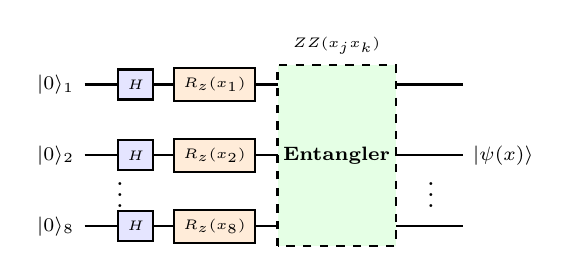
\begin{tikzpicture}[>=stealth, thick, node distance=1.2cm]
                \draw (0, 1.8) node[left] {\scriptsize $|0\rangle_1$} -- (4.8, 1.8);
                \draw (0, 0.9) node[left] {\scriptsize $|0\rangle_2$} -- (4.8, 0.9);
                \draw (0, 0.0) node[left] {\scriptsize $|0\rangle_8$} -- (4.8, 0.0);
                
                \node at (0.45, 0.5) {$\vdots$};
                \node at (4.4, 0.5) {$\vdots$};

                \node[draw, fill=blue!10, minimum size=0.38cm] at (0.65, 1.8) {\tiny $H$};
                \node[draw, fill=blue!10, minimum size=0.38cm] at (0.65, 0.9) {\tiny $H$};
                \node[draw, fill=blue!10, minimum size=0.38cm] at (0.65, 0.0) {\tiny $H$};

                \node[draw, fill=orange!15, minimum size=0.38cm] at (1.65, 1.8) {\tiny $R_z(x_1)$};
                \node[draw, fill=orange!15, minimum size=0.38cm] at (1.65, 0.9) {\tiny $R_z(x_2)$};
                \node[draw, fill=orange!15, minimum size=0.38cm] at (1.65, 0.0) {\tiny $R_z(x_8)$};

                \draw[fill=green!10, dashed] (2.45, -0.25) rectangle (3.95, 2.05);
                \node at (3.2, 0.9) {\scriptsize \textbf{Entangler}};
                \node[above] at (3.2, 2.05) {\tiny $ZZ(x_j x_k)$};
                
                \node[right] at (4.8, 0.9) {\scriptsize $|\psi(x)\rangle$};
            \end{tikzpicture}
            }
        \end{block}

        \vspace{-0.2cm}
        \begin{block}{\scriptsize Data Pipeline \& Dual Solver}
            \centering
            \resizebox{0.92\textwidth}{!}{
            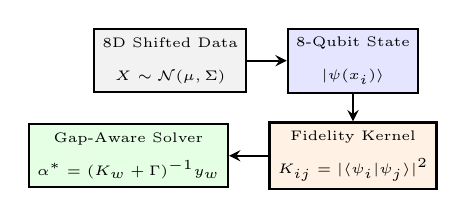
\begin{tikzpicture}[>=stealth, thick, auto, node distance=0.7cm]
                \node[draw, rectangle, fill=gray!10, align=center, inner sep=3pt] (tensor) {\tiny 8D Shifted Data\\ \tiny $X \sim \mathcal{N}(\mu, \Sigma)$};
                \node[draw, rectangle, fill=blue!10, right=0.5cm of tensor, align=center, inner sep=3pt] (qstate) {\tiny 8-Qubit State\\ \tiny $|\psi(x_i)\rangle$};
                \node[draw, rectangle, fill=orange!10, below=0.35cm of qstate, align=center, inner sep=3pt] (gram) {\tiny Fidelity Kernel\\ \tiny $K_{ij} = |\langle\psi_i|\psi_j\rangle|^2$};
                \node[draw, rectangle, fill=green!10, left=0.5cm of gram, align=center, inner sep=3pt] (qkrr) {\tiny Gap-Aware Solver\\ \tiny $\alpha^* = (K_w + \Gamma)^{-1}y_w$};

                \draw[->] (tensor) -- (qstate);
                \draw[->] (qstate) -- (gram);
                \draw[->] (gram) -- (qkrr);
            \end{tikzpicture}
            }
        \end{block}
    \end{column}
\end{columns}
\end{frame}

% ---------------------------------------------------------
% SLIDE 2: RESEARCH QUESTION AND TENTATIVE TIMELINE
% ---------------------------------------------------------
\begin{frame}{Research question and tentative timeline}
\vspace{-0.3cm}
\begin{columns}[T]
    % Left Column: Problem, Theory & Algorithmic Contributions
    \begin{column}{0.54\textwidth}
        \begin{itemize}\setlength{\itemsep}{2pt}
            \item \textbf{What Problem Are You Asking?}
            \begin{itemize}\setlength{\itemsep}{1pt}
                \item Why does provable quantum advantage in QKRR collapse out-of-sample under covariate shift?
                \item \textbf{Mechanism:} Distribution shift $\mu \to \tilde{\mu} \implies \Sigma_{\tilde{\mu}} = \Sigma_\mu + V$ on RKHS. Exponential spectral concentration forces $\delta \approx 0$, causing Davis-Kahan rotation $\frac{\|V\|}{\delta} \to \infty$ to scramble coordinate axes and destroy out-of-sample risk.
            \end{itemize}

            \item \textbf{Scope, Assumptions \& Contributions:}
            \begin{itemize}\setlength{\itemsep}{1pt}
                \item \textbf{Assumptions:} Covariate shift ($P_{\text{train}}(x) \neq P_{\text{test}}(x)$), self-adjoint compact covariance operators $\Sigma_\mu, \Sigma_{\tilde{\mu}} \in \mathcal{S}_\infty(\mathcal{H})$.
                \item \textbf{Theory (Step 1):} Caponnetto--De Vito RKHS excess risk bound $\|f^* - f_0\|_{L^2(\tilde{\mu})}^2$ explicitly parameterized by $\delta$ and $\|V\|$.
                \item \textbf{Algorithm (Steps 2--3):} Gap-Aware Regularizer $\Gamma = \operatorname{diag}(\lambda / \delta_j^2)$ + density reweighting $w(x) = \frac{P_{\text{test}}(x)}{P_{\text{train}}(x)}$ to suppress unstable tail modes.
            \end{itemize}
        \end{itemize}
    \end{column}

    % Right Column: Subspace Rotation Flowchart & Semester Timeline
    \begin{column}{0.44\textwidth}
        \vspace{-0.1cm}
            \begin{block}{\scriptsize Subspace Rotation Failure Mechanism}
        \centering
        \resizebox{0.92\textwidth}{!}{
        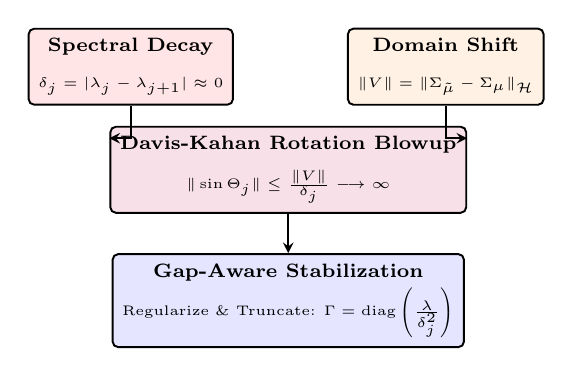
\begin{tikzpicture}[
            >=stealth, 
            thick, 
            auto,
            block/.style={
                draw, 
                rectangle, 
                rounded corners=2pt,
                align=center, 
                inner sep=3.5pt, 
                line width=0.7pt
            }
        ]
            \node[block, fill=red!10] (decay) at (-2.0, 0) {
                \scriptsize \textbf{Spectral Decay}\\[1pt] 
                \tiny $\delta_j = |\lambda_j - \lambda_{j+1}| \approx 0$
            };
            
            \node[block, fill=orange!10] (shift) at (2.0, 0) {
                \scriptsize \textbf{Domain Shift}\\[1pt] 
                \tiny $\|V\| = \|\Sigma_{\tilde{\mu}} - \Sigma_\mu\|_{\mathcal{H}}$
            };
    
            \node[block, fill=purple!12, below=0.75cm of $(decay)!0.5!(shift)$] (rot) {
                \scriptsize \textbf{Davis-Kahan Rotation Blowup}\\[2pt] 
                \tiny $\|\sin\Theta_j\| \le \frac{\|V\|}{\delta_j} \longrightarrow \infty$
            };
    
            \node[block, fill=blue!10, below=0.5cm of rot] (fix) {
                \scriptsize \textbf{Gap-Aware Stabilization}\\[2pt] 
                \tiny Regularize \& Truncate: $\Gamma = \operatorname{diag}\left(\frac{\lambda}{\delta_j^2}\right)$
            };
    
            % Clean side routing entering the lateral anchors of the middle box
            \draw[->, line width=0.7pt] (decay.south) |- (rot.170);
            \draw[->, line width=0.7pt] (shift.south) |- (rot.10);
            \draw[->, line width=0.7pt] (rot.south) -- (fix.north);
        \end{tikzpicture}
        }
    \end{block}

        \vspace{-0.15cm}
        \begin{block}{\scriptsize Deliverables \& Timeline (Autumn 2026)}
            \tiny
            \textbf{14--15 Sep (Pres. 2):} Analytical excess risk bound derivation parameterized by $(\delta, \|V\|)$; baseline QKRR replication.\\
            \textbf{26--27 Oct (Pres. 3):} Dual Gap-Aware solver implementation; 8-qubit IQP benchmark verification.\\
            \textbf{16--17 Nov (Pres. 4):} Multi-model benchmarking vs Classical RBF/XGBoost \& final 2-page report.
        \end{block}
    \end{column}
\end{columns}
\end{frame}

\end{document}